\documentclass[12pt, letterpaper]{report}
\usepackage{graphicx}
\usepackage{hyperref}
\usepackage{amssymb}
\usepackage{amsmath}
\usepackage{float}
\usepackage{mathtools}
\usepackage{enumitem}
\usepackage[margin=1in]{geometry}
\usepackage[figurename=Figura]{caption}
\title{Ley de Coulomb}
\author{Juan Pablo Guerrero Escudero}
\date{01 abril, 2024}
\begin{document}
\maketitle
\textbf{Electromagnetismo}: Inició aproximadamente en 1800. En el curso, serán 2 semanas de Electroestática, 
y dos semanas de Magnetoestática. \\

Unidades de éste módulo
\begin{enumerate}
\item SI o Sistema Internacional (kg, m, s, k)
\item CGS (cm, g, s). 
\end{enumerate}
En el CGS no hay constante de proporcionalidad, en el SI sí lo hay.
\subsection*{Ley de Coulomb}
En electromagnetismo usualmente mides la carga eléctrica. Entonces, con la ley de Coulomb puedes medir 
la fuerza entre cargas eléctricas. Ésta ley experimental nos dice que las cargas opuestas se \textbf{atraen} y 
que las cargas similares se \textbf{repelen}. \\
Existe una fuerza de atracción entre dos cargas a lo largo de una recta que las une (r): 
\begin{figure}[H]
    \centering
    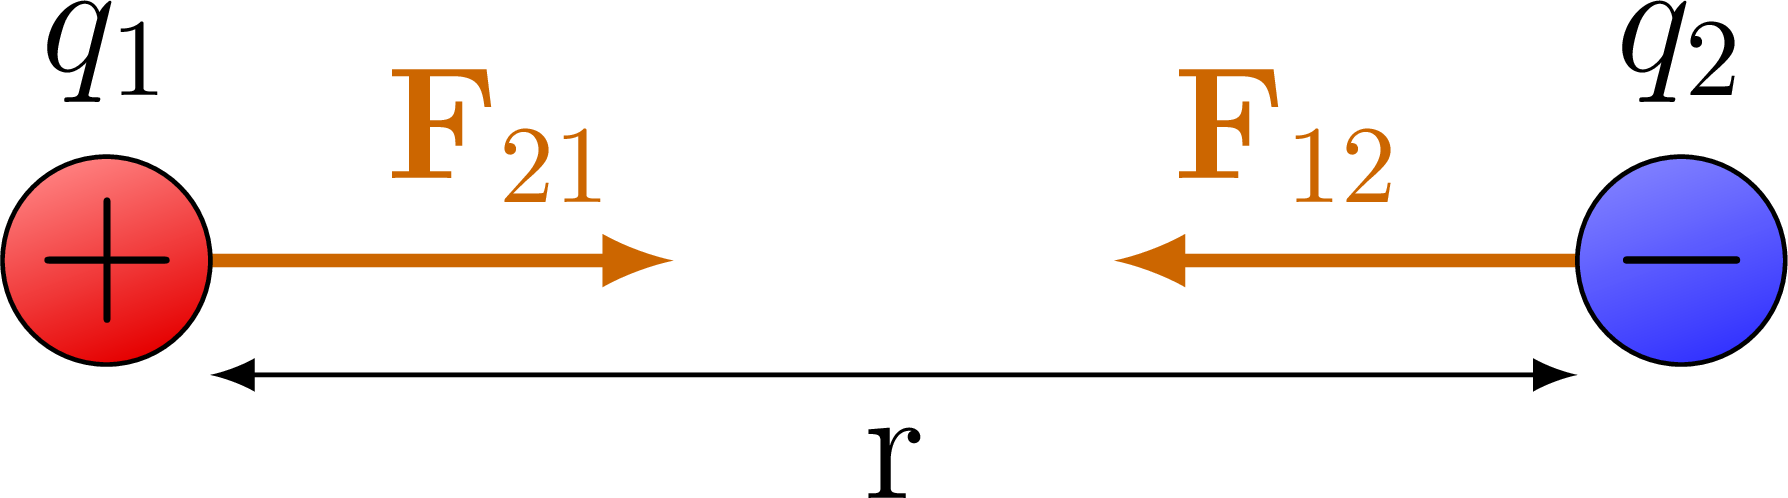
\includegraphics[height = 2cm]{coulomb_force.png}
    \caption{Representación Ley de Coulomb}
\end{figure}
Obs: la fuerza \textbf{siempre} va en la dirección de la línea que une las cargas. \\
Después, la ley de Coulomb dice que la Fuerza es directamente proporcional al producto de las cargas $Q_1$ y $Q_2$, y 
es inversamente proporcional al cuadrado de la distancia $R^2$ entre ellas. 

Entonces la fórmula es: 
\begin{align*}
F \propto& k(\frac{Q_1Q_2}{R^2}) \\ 
F =& (\frac{1}{4\pi \epsilon_0})(\frac{Q_1Q_2}{R^2}). \\
\end{align*}
Aquí, $\epsilon_0$ representa la permitividad del vacío. La fórmula de Fuerza se mide en Newtons. \\
Ahora, como la Fuerza es un vector, necesita la dirección también ($\vec{F}$), entonces: 
\begin{align*}
    \vec{F} = (\frac{1}{4\pi \epsilon_0})(\frac{Q_1Q_2}{R^2})(\hat{a}_R). 
\end{align*} Donde $\hat{a}_R$ es el vector unitario, es decir $|\hat{a}_R| = 1$. \\

\textbf{Vector Separación}: El vector separación $\vec{R}$ es el vector de la distancia entre dos cargas. Se calcula 
de la siguiente manera: $\vec{R} = \vec{R_2} - \vec{R_1}$, siendo $\vec{R}_2$ y $\vec{R}_1$ el vector desde el origen 
a cada carga $Q_1$ y $Q_2$.
\begin{figure}[H]
    \centering
    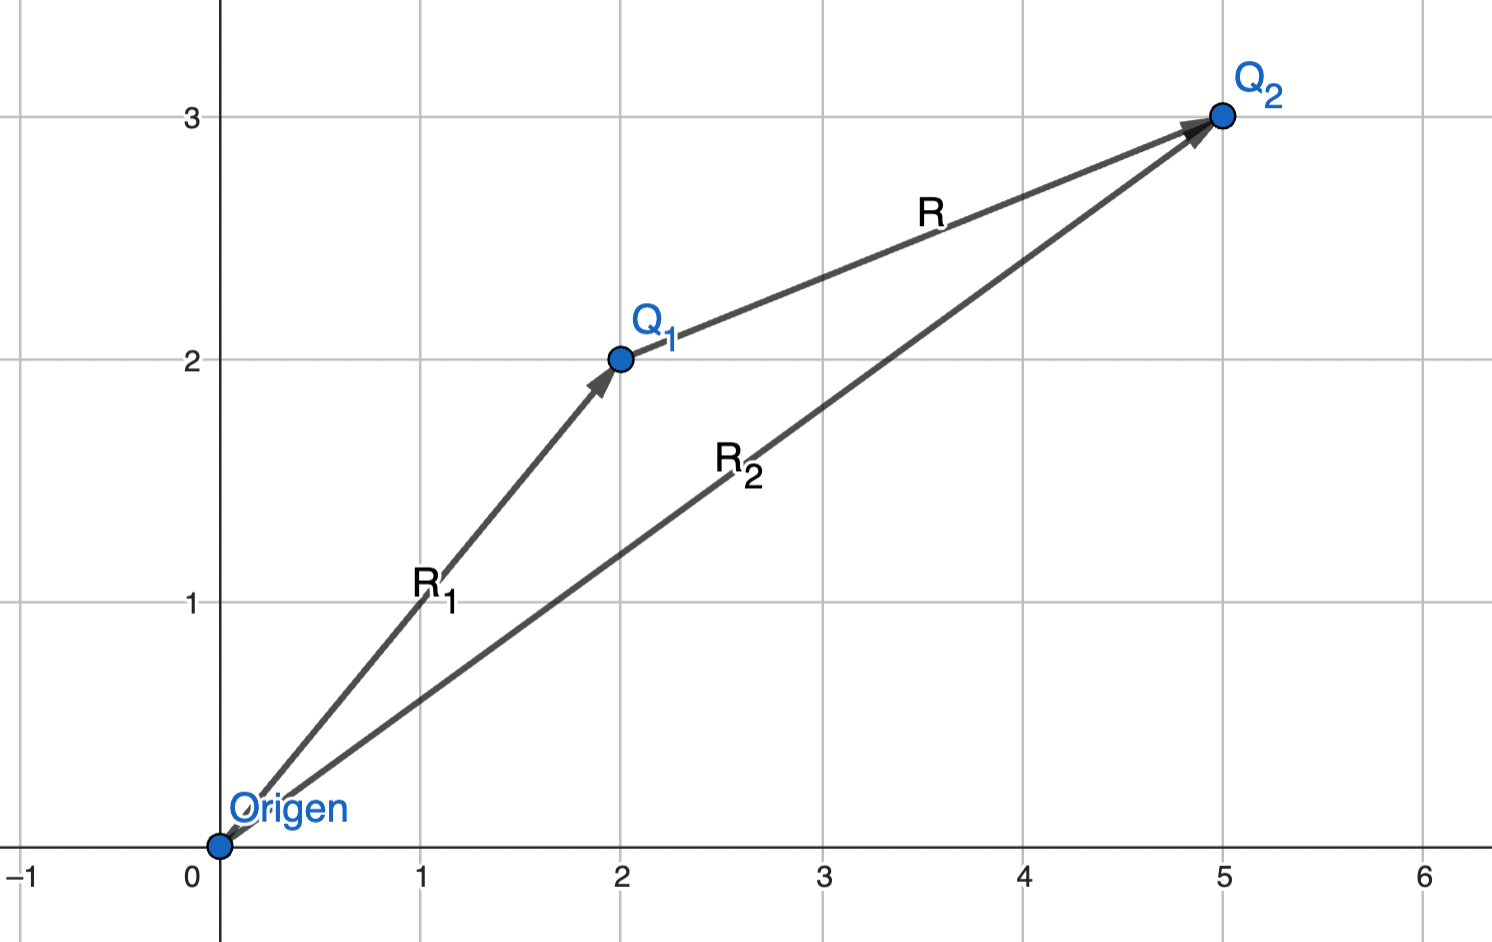
\includegraphics[height = 6cm]{SeparationVector.png}
    \caption{Vector $\vec{R}$ de separación}
\end{figure}
Se puede intuir la fórmula usando el cálculo vectorial, reconociendo que $\vec{R_1} + \vec{R} = \vec{R_2}$, y despejando 
$\vec{R} = \vec{R_2} - \vec{R_1}$. Para saber cuál restar primero, se resta el vector donde "llegas" menos el vector "de donde sales". \\

Después, se puede calcular la separación entre las cargas, la cuál es $|\vec{R}| = R$., y por lo tanto el vector unitario 
$\hat{a}_R = \frac{\vec{R}}{R}$, donde $\vec{R}$ es el vector y $R$ es la magnitud. \textbf{Obs}: Se utilizan vectores unitarios 
para dejar la fuerza intacta. Entonces, la fórmula final de la Ley de Coulomb resulta: 
\begin{align*}
\vec{R} =& (\frac{1}{4\pi \epsilon_0})(\frac{Q_1Q_2}{R^2})(\frac{\vec{R}}{R}) \\
\vec{R} =& (\frac{1}{4\pi \epsilon_0})(\frac{Q_1Q_2}{R^3})(\vec{R})
\end{align*}\\
\textbf{Principio de superposición}: 
$\vec{F_1} + \vec{F_2} + \vec{F_3} + \vec{F_n} = \vec{F_{neta}}$. 
\end{document}